\chapter{Succinct Self-Index}
\lhead{Chapter 4. \emph{Succinct Self-Index}} % this is for the header on each page - perhaps a shortened title

As performance of inverted list based search engine is limited by disk I/O, we build a in-memory one to provide much higher throughput based on the family of
succinct data structures. Most available solutions for succinct in-memory index can be classified into two categories: compressed suffix array(CSA) and FM-index.
Both use wavelet trees to store data and support three basic operations: \(access\), \(rank\) and \(select\). Our solution is based on FM-index and document array. It
trades long build time and large memory consumption for low latency and high concurrency.


\section{One Cache-miss Bitvector}

A wide variety of succinct data structures are build upon wavelet trees, each node of which is a bitvector (or integer vector for multi-ary wavelet trees). The three bitvector
operations --- access, rank and select --- are fundamental for algorithms on wavelet trees. Figure \ref{fig:rankselect} shows the definition of a rank/select operation
on a basic bitvector. Thus a carefully designed bitvector with good performance is crucial for a fast succinct index solution. In our implementation major part of computation
occurs on document array. To maximize the performance of retrieval algorithms, we designed one cache-miss bitvector for document array.

\begin{figure}[h!]
\centerline{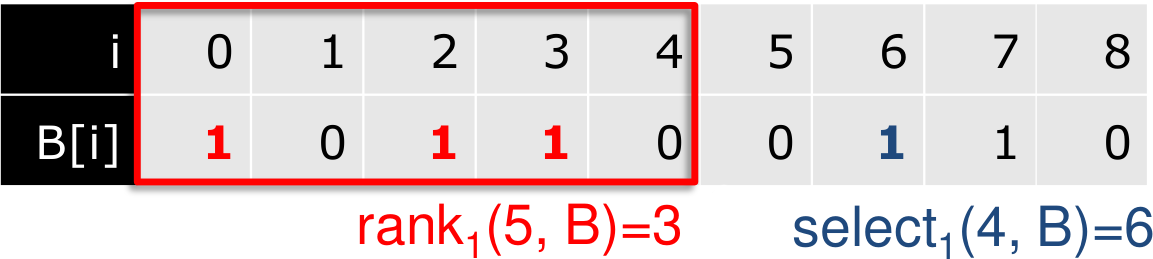
\includegraphics[width=0.6\textwidth]{Figures/rankselect.png}}
\caption{Rank/Select Operation of a Bitvector}\label{fig:rankselect}
\end{figure}


\subsection{Data Structure}
The design of bitvector with rank/select operation supported is to struggle with cache misses, during a retrieval process over wavelet trees, there are intensive rank operations
getting involved, as a result, the number of cache misses is one of major bottleneck for performance improvements since the complexity of wavelet trees is optimal. A general
design of bitvector will introduce 4-6 cache misses for each rank operation, and there are several research works to reach state-of-the-art results on reducing cache misses,
such as \cite{gog2013optimized}, \cite{zhou2013space}, which claimed to have 2 to 3 cache misses for each rank operation, see in figure \ref{fig:cachemisses}.

\begin{figure}[h!]
\centerline{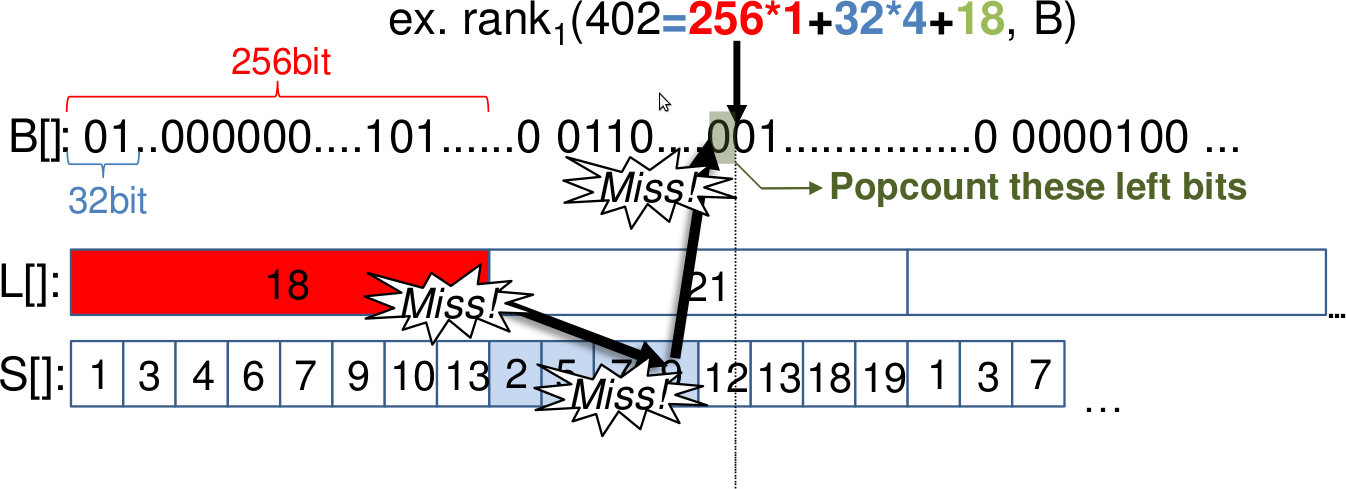
\includegraphics[width=0.6\textwidth]{Figures/cachemisses.png}}
\caption{3 Cache/TLB Misses Per Rank of a Bitvector}\label{fig:cachemisses}
\end{figure}


Our solution is to split the original data into blocks of 384 bits (uint64\_t[6]), then for each block we store the rank value for its initial position and the partial rank values of each 64-bit integer. The partial rank values are stored like this: each partial value is not more than 384 (9 bits), and each block has 7 partial values, so we need at least \(9*7=63\) bits which can be compacted into a 64-bit integer. Thus each block is exactly 512 bits. Answering a rank() query, we calculate the block index and offset, and sum up the initial rank of that block, the partial rank of one particular integer and the popcount of part of that integer, all of which reside in a single cache line inferring exact one cache miss.

The structure of a super block looks like below:
\begin{lstlisting}
struct SuperBlock
{
    uint64_t rank_;
    uint64_t subrank_;
    uint64_t bits_[6];
};
\end{lstlisting}

\subsection{Rank Query}

It is convenient to calculate \(rank\) value on one cache-miss bitvector. First we calculate the superblock and block indexes for queried position. Then the \(rank\) value is
\begin{align*}
  rank_1(pos) &= sb[sb\_index(pos)].rank\_ \\
              &+ (sb[sb\_index(pos)].subrank\_ >> (9 * b\_index(pos)) | 511) \\
              &+ popcount(mask(sb[sb\_index(pos)].bits\_[b\_index(pos)], b\_offset(pos)))
\end{align*}

\section{Wavelet tree}

The Wavelet Tree is a succinct data structure to store strings in compressed space. Wavelet Tree converts a string into a balanced binary-tree of bit vectors, where a 0 replaces half of the symbols, and a 1 replaces the other half. This creates ambiguity, but at each level this alphabet is filtered and re-encoded, so the ambiguity lessens, until there is no ambiguity at all.
The tree is defined recursively as follows:

\ \ \ \ 1. Take the alphabet of the string, and encode the first half as 0, the second half as 1, for example, {a,b,c,d} would become {0,0,1,1};

\ \ \ \ 2. Group each 0-encoded symbol, {a,b}, as a sub-tree;

\ \ \ \ 3. Group each 1-encoded symbol, {c,d}, as a sub-tree;

\ \ \ \ 4. Reapply this to each subtree recursively until there is only one or two symbols left (when a 0 or 1 can only mean one thing).

For the string \('Peter Piper picked a peck of pickled peppers'\) (spaces and a string terminator have been represented as \_ and \$ respectively, due to convention in the literature) the Wavelet Tree would look like this in Table \ref{ex:awt}. Note that the strings aren’t actually stored, but are shown here for convenience.

\begin{table}[!htp]
  \caption{A Wavelet Tree}
  \label{ex:awt}
  \begin{center}
    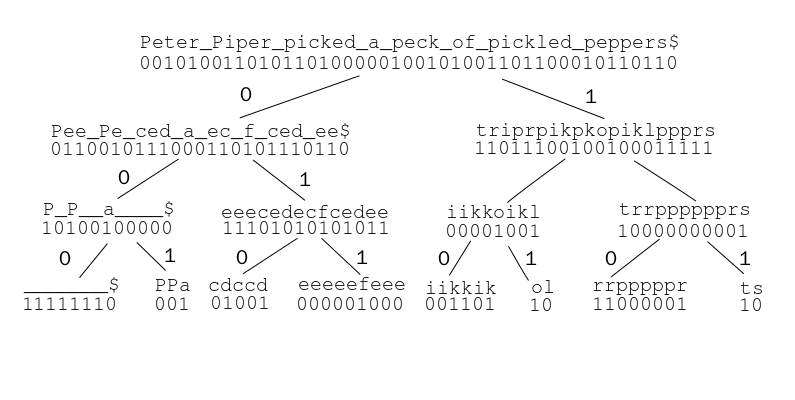
\includegraphics[width=1\textwidth]{Figures/graph1.png}
  \end{center}
\end{table}

It has the alphabet \(\{\$,P,_,a,c,d,e,f,i,k,l,o,p,r,s,t\}\), which would be mapped to \(\{0,0,0,0,0,0,0,0,1,1,1,1,1,1,1,1\}\). So, for example, \$ would map to 0, and r would map to 1.

The left subtree is created by taking just the 0-encoded symbols \(\{\$,P,_,a,c,d,e,f\}\) and then re-encoding them by dividing this new alphabet: \(\{0,0,0,0,1,1,1,1\}\). Note that on the first level an e would be encoded as a 0, but now it is encoded as a 1 (it becomes a 0 again at a leaf node).

In fact, since it is a balanced tree, we can concatenate each of the levels and store it as one single bit vector.
Actually, the data structure we used is a variant of Wavelet Tree named Wavelet Matrix, which introduced by (Claude el at,. 2012 \cite{claude2012}).
The idea of the Wavelet Matrix is to break the assumption that the children of a node v at interval \([s,e]\), must be aligned to it and occupy the same interval in the next level. Freeing the structure from this unnecessary assumption allows us to design a much simpler mapping mechanism from one level to the next: all the 0s of the level go left, and all the 1s go right. For each level, we will store a single integer \(z[l]\) that tells the number of 0s in level \(l\).

\subsection{Rank in Wavelet Tree}

A rank query is the count of 1-bits up to a specified position. Rank queries over larger alphabets are analogous – instead of a 1, it may be any other symbol.
After the tree is constructed, a rank query can be done with \(O(logA)\) (A is alphabet size) binary rank queries on the bit vectors in \(O(1)\)(Claude et al., 2008 \cite{claude2008}). The encoding at each internal node may be ambiguous, but of course it isn’t useless – we use the ambiguous encoding to guide us to the appropriate sub-tree, and keep doing so until we have our answer.

For example in Table \ref{ex:riwt}, if we wanted to know \(rank(5,e)\), we use the following procedure which is illustrated below. We know that \(e\) is encoded as 0 at this level, so we take the binary rank query of 0 at position 5. Which is 4, which we then use to indicate where to rank in the 0-child: the 4th bit (or the bit at position 3, due to 0-basing). We know to query the 0-child, since that is what e was encoded as at the parent level. We then repeat this recursively. At a leaf node we have our answer.

\begin{table}[!htp]
  \caption{Rank in Wavelet Tree}
  \label{ex:riwt}
  \begin{center}
    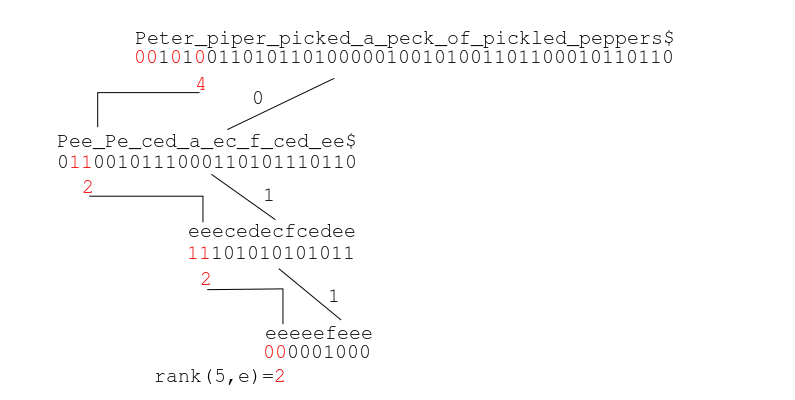
\includegraphics[width=1\textwidth]{Figures/graph2.png}
  \end{center}
\end{table}

\section{FM-Index}

FM-index(Full-text index in Minute space) is a compressed full-text substring index based on the Burrows-Wheeler Transform, with some similarities to the suffix array. It was created by (Paolo et al., 2001 \cite{paolo2001}) who describe it as an opportunistic data structure as it allows compression of the input text while still permitting fast substring queries.
It can be used to efficiently find the number of occurrences of a pattern within the compressed text, as well as locate the position of each occurrence. Both the query time and storage space requirements are sublinear with respect to the size of the input data. In contrast, the FM-index is a compressed self-index, which means that it compresses the data and indexes it at the same time.

\subsection{Suffix Arrays}

There is a variety of Suffix Array construction algorithms, including some \(O(N)\) ones (Puglisi et al., 2007 \cite{puglisi2007}). However, we will explain it from the most common (and intuitive) angle. In its simplest form, a suffix array can be constructed for a string \(S[1..N]\) like so:

\ \ \ \ 1. Construct an array of pointers to all suffixes \(S[1..N],S[2..N],…,S[N..N]\).

\ \ \ \ 2. Sort these pointers by the lexicographical (i.e. alphabetical) ordering of their associated suffixes.

For example, the sorting of the string \('abracadabra'\) with terminating character '\$' would look like this in Table \ref{ex:gsa}:

\begin{table}[!htp]
  \caption{Get Suffix Array}
  \label{ex:gsa}
  \begin{center}
    \begin{tabular}{c|c|c|c}
      \hline
      \hline
      index & string & sa & string \\
      \hline
      1 & abracadabra\$ & 12 & \$ \\
      \hline
      2 & bracadabra\$ & 11 & a\$ \\
      \hline
      3 & racadabra\$ & 8 & abra\$ \\
      \hline
      4 & acadabra\$ & 1 & abracadabra\$ \\
      \hline
      5 & cadabra\$ & 4 & acadabra\$ \\
      \hline
      6 & adabra\$ & 6 & adabra\$ \\
      \hline
      7 & dabra\$ & 9 & bra\$ \\
      \hline
      8 & abra\$ & 2 & bracadabra\$ \\
      \hline
      9 & bra\$ & 5 & cadabra\$ \\
      \hline
      10 & ra\$ & 7 & dabra\$ \\
      \hline
      11 & a\$ & 10 & ra\$ \\
      \hline
      12 & \$ & 3 & racadabra\$ \\
      \hline
    \end{tabular}
  \end{center}
\end{table}

\subsection{Burrows-Wheeler Transform}

The Burrows-Wheeler Transform (BWT) is a was developed by Burrows and Wheeler to reversibly permute a string in such a way that characters from repeated substrings would be clustered together. It was useful for compression schemes such as run-length encoding.
It is not the point of this article to explain how it works, but it is closely linked to Suffix Arrays: \(BWT[i] = S[SA[i] {-} 1]\), for the original string S, suffix array SA, and Burrows-Wheeler Transform string BWT. In other words, the ith symbol of the BWT is the symbol just before the ith suffix.
The BWT also lets us reconstruct the original string S, allowing us to discard the original document – indexes with this property are known as self indexes, which introduced by (Paolo et al., 2005 \cite{paolo2005}).

An FM-index is created by first taking the BWT of the input text. For example, the BWT of the string T = "abracadabra" is "ard\$rcaaaabb", and here it is represented by the matrix M in Table \ref{ex:mm} where each row is a rotation of the text that has been sorted. The transform corresponds to the last column labeled L.

\begin{table}[!htp]
  \caption{Matrix M}
  \label{ex:mm}
  \begin{center}
    \begin{tabular}{c|c|c}
      \hline
      \hline
      F & String & L \\
      \hline
      \$ & abracadabr & a \\
      \hline
      a & \$abracadab & r \\
      \hline
      a & bra\$abraca & d \\
      \hline
      a & bracadabra & \$ \\
      \hline
      a & cadabra\$ab & r \\
      \hline
      a & dabra\$abra & c \\
      \hline
      b & ra\$abracad & a \\
      \hline
      b & racadabra\$ & a \\
      \hline
      c & adabra\$abr & a \\
      \hline
      d & abra\$abrac & a \\
      \hline
      r & a\$abracada & b \\
      \hline
      r & acadabra\$a & b \\
      \hline
    \end{tabular}
  \end{center}
\end{table}

The BWT in itself allows for some compression with, for instance, move to front and Huffman encoding, but the transform has even more uses. The rows in the matrix are essentially the sorted suffixes of the text and the first column F of the matrix shares similarities with suffix arrays. How the suffix array relates to the BWT lies at the heart of the FM-index.

It is possible to make a last-to-first column mapping \(LF(i)\) from a character \(L[i]\) to \(F[j]\), with the help of a table \(C[c]\) and a function \(Occ(c, k)\). \(C[c]\) is a table that, for each character c in the alphabet, contains the number of occurrences of lexically smaller characters in the text. The function \(Occ(c, k)\) is the number of occurrences of character c in the prefix \(L[1..k]\). (Paolo et al., 2005 \cite{paolo2005}) showed that it is possible to compute \(Occ(c, k)\) in constant time.

The last-to-first mapping can now be defined as \(LF(i) = C[L[i]] + Occ(L[i], i)\). For instance, on row 9, \(L\) is a and the same a can be found on row 5 in the first column \(F\), so \(LF(9)\) should be 5 and \(LF(9) = C[a] + Occ(a, 9) = 5\). For any row i of the matrix, the character in the last column \(L[i]\) precedes the character in the first column \(F[i]\) also in T. Finally, if \(L[i] = T[k]\), then \(L[LF(i)] = T[k - 1]\), and using the equality it is possible to extract a string of \(T\) from \(L\).

The FM-index itself is a compression of the string \(L\) together with \(C\) and \(Occ\) in some form, as well as information that maps a selection of indices in \(L\) to positions in the original string \(T\).

\section{Fuzzy-Search Algorithms}

Let's briefly introduce our search algorithms. When we get a search query, we divide it to several terms. Each term is given a score, correspond to it's significance. Then search each term in FM-Index to get it's range. Do union operation with all term's range, and get K most related result as our final result.

\subsection{Build FM-Index}

We have \(N\) documents in our database whose text is \(t1,t2...tN\), \(T\) is contection of these text with terminating character \(\$\) for each text, as \(T=t1\$t2\$...tN\$\). Do BWT with \(T\) could get a FM-Index stored in Wavelet Tree, our searching based on this data structure.

\subsection{Get terms from search query}

Search query should be tokenize into terms, and we use the vector of terms to do next operation. Score terms would help us to rank the search result, higher score means more significance. For example, query is 'white shirt', 'shirt' have higher score than 'white', result contains only 'shirt' would rank higher than that contains only 'white' because we prefer 'yellow shirt' than 'white car'. It's just a small part of rank, we won't discuss more about rank in this article. Terms in a dictionary of brand\&good have the highest score, terms in a usual dictionary have lower score, terms construction as bigram or others have the lowest score.

\subsection{Backward search for each term}

Since any pattern \(P\) in \(S\) (the original string) is a prefix of a suffix (our Suffix Array stores suffixes), and the suffixes are lexicographically ordered, all occurrences of a search pattern \(P\) lie in a contiguous portion of the Suffix Array.
Backward search instead utilises the BWT in a series of paired rank queries (which can be answered with a Wavelet Tree), improving the query performance considerably. Backward search issues p pairs of rank queries, where p denotes the length of the pattern P. The paired rank queries are:

\begin{equation}
  \label{ex:equation_bs}
  \begin{aligned}
    &s' = C[P[i]] + rank(s {-} 1, P[i]) + 1 \\
    &e' = C[P[i]] + rank(e, P[i])
  \end{aligned}
\end{equation}

\(C\) is a lookup table containing the count of all symbols in our alphabet which sort lexicographically before \(P[i]\).
Where \(s\) denotes the start of the range and \(e\) is the end of the range. Initially \(s=1\) and \(e=N\). Index variable \(i\) starts at \(p\), decreases to 1, then get the answer. If \(e<s\) at any stage, then \(P\) doesn’t exist in \(S\). This maintains the invariant that \(SA[s..e]\) contains all the suffixes of which \(P[i..|P|]\) is a prefix, and hence all locations of \(P[i..|P|]\) in \(S\).
After backward searching, we get \([left\_range, right\_range, score]\) for each term(score get in last step), we could get the most related documents from the range set then.

\subsection{Top K Union}

Union opeartion with the range set after backward searching could get documents set which contains all terms. But in most cases, there is no document hits all terms in query, thus we want to get the document which have higher score that means higher relevance with the query. We name this operation 'top k union', as will get top k most related result after union.

Naive top k union is easy, pseudo code looks like this, then sort \(doc[]\) we could get the most related documents.

\begin{scriptsize} \begin{verbatim}
for j = 1 to range_set_size
    for i = range[j]'s left_range to range[j]'s right_range
        doc[i]'s score += score[j];
\end{verbatim} \end{scriptsize}

The time complexity is \[O(range\_set\_size\ *\ (range\_right\ -\ range\_left)) + O(sort\ all\ documents)\] and space complexity is \(O(document\ number)\), assume we have N = 100 million document, \(range\_right - range\_left\) could be at most \(N\), and a query contains at most 20 terms, the time complexity is \(O(10^8 * 20)\) and space complexity is \(O(10^8)\), both is too large.

Do you remember the Wavelet Tree? It perform perfect in backward search, and combined with heuristic searching, it could give us a excellent solution in top k union also.

Retrieve data structure of the Wavelet Tree in FM-Index, tree's root stores all text's BWT, partition it level by level, and leaf denotes document.
We define 'status' by a range set, a tree node, and a score, that means in the current node, ranges in the range set is available, and the score is the sum of all available ranges. For example, the initial status's range set is the range set after backward search which corresponding each term, node is tree's root, that means all range is available for the root, score is the sum of all terms in query.
For each status, we could derive status from it. Range will be partition into 2 ranges in the next level, one for 0 and another for 1, corresponding node is current node's left child and right child. Sometimes a derived status have a \(NULL\) range set, we should drop this status because no documents hit any terms in this node's subtree.
Every time we choose a status with highest score to derive, when status' node is a leaf, we get one result document. It's easy to find that the nth document we get has the nth highest score. It will be stopped when we get k document or all status has been derived. That is the mainly meaning of 'fuzzy search', when couldn't find document hits all terms, we could get the top k most related. Of course the document hits all terms have the highest score and won't be losen.

Pruning in searching is needed as the intermediate result is too large, we use a interval heap which key is score to store status, that could help us to get the status with highest/lowest score in \(O(1)\), and heap size is delimited to specified \(MAX\_SIZE\), when heap size reaches \(MAX\_SIZE\), we can replace the status with lowest score to a new status in \(O(log(MAX\_SIZE))\).
Pseudo code of top k union looks like follow.

\begin{scriptsize} \begin{verbatim}
heap_insert(original_range_set, root);
while(result_size < k)
{
    top_status = heap_get_max();
    if (top_status->root == leaf)
    {
        result_add(top_status);
    }
    else
    {
        for i = 0 to top_status->range_size
        {
            left/right_range = get left/right child range from top_status;
            if (left/right_range != NULL)
            {
                add left/right_range to left/right_status;
                add range's score to left/right_status;
            }
        }

        if (left/right_status != NULL and heap->size < MAX_SIZE)
            heap_insert(left/right_range);
        else if (left/right_range->score > heap_get_min()->score)
            heap_replace_min(left/right_range);
    }
}
\end{verbatim} \end{scriptsize}

\(Get\ left/right\ child\ range\) operation cost constant time as rank in a Wavelet Tree's node cost constant. We have to do it \(range\_set\_size\) times for each status, and status number is up to node number in the Wavelet Tree, equals to \(2*N\). The time complexity is \(O(range\_set\_size * N)\).
We have to store \(range\_set\_size\) ranges for each status, and status in interval heap is up to \(MAX\_SIZE\), space complexity is \(O(range\_set\_size * MAX\_SIZE)\).
It seems that time complexity is large than the naive version, but in parctise, as used pruning, status we traversed is much less than \(N\), usually less than \(N/20\). In practise we set \(MAX\_SIZE\) to \([1000..10000]\), the space complexity is much smaller than the naive version too.

\subsection{Major and Minor Terms}

Major and minor feature is used for getting better result in searching. After setting score for each term, we move significant terms(often with high score) into major set and the rest into minor set. Each returned doc contains all the major terms and any number of minor terms, thus this is a half-intersection half-union algorithm. The intersection part makes bare branches pruned much faster so that entire search performance accelerated by 3 times.

Pseudo code of the improved top k union looks like follow.

\begin{scriptsize} \begin{verbatim}
heap_insert(original_range_set, root);
while(result_size < k)
{
    top_status = heap_get_max();
    if (top_status->root == leaf)
    {
        result_add(top_status);
    }
    else
    {
        for i = 0 to top_status->major_size
        {
            left/right_range = get left/right child range from top_status;
            if (left/right_status != NULL && left/right_range != NULL)
            {
                add left/right_range to left/right_status;
                add range's score to left/right_status;
            }
            else
            {
                left/right_status = NULL;
            }
        }

        for i = top_status->major_size to top_status->range_size
        {
            left/right_range = get left/right child range from top_status;
            if (left/right_status != NULL && left/right_range != NULL)
            {
                add left/right_range to left/right_status;
                add range's score to left/right_status;
            }
        }

        if (left/right_status != NULL and heap->size < MAX_SIZE)
            heap_insert(left/right_range);
        else if (left/right_range->score > heap_get_min()->score)
            heap_replace_min(left/right_range);
    }
}
\end{verbatim} \end{scriptsize}

\subsection{Synonym}

Synonym searching means that we could get result documents which hits the synonym of term. For example, text contains only 'LV bag', query is 'Louis Vuitton bag', we could get it under synonym searching, obviously it missing in normal searching.

We build a dictionary of synonym from the SCD first, that will help us to expand original term to a synonym term set for each term, set synonym's score little lower than the original one. Then do backward search with new term set.
In top k union, we calculate status' score for each synonym term set once, that means if more than one term in the same synonym set hit a status, only the highest score will be added.
